\documentclass{beamer}
\mode<presentation>
\usepackage{amsmath}
\usepackage{amssymb}
%\usepackage{advdate}
\usepackage{adjustbox}
\usepackage{subcaption}
\usepackage{enumitem}
\usepackage{multicol}
\usepackage{mathtools}
\usepackage{listings}
\usepackage{url}
\def\UrlBreaks{\do\/\do-}
\usetheme{AnnArbor}
\usecolortheme{spruce}
\setbeamertemplate{footline}
{
  \leavevmode%
  \hbox{%
  \begin{beamercolorbox}[wd=\paperwidth,ht=2.25ex,dp=1ex,right]{author in head/foot}%
    \insertframenumber{} / \inserttotalframenumber\hspace*{2ex} 
  \end{beamercolorbox}}%
  \vskip0pt%
}
\setbeamertemplate{navigation symbols}{}

\providecommand{\nCr}[2]{\,^{#1}C_{#2}} % nCr
\providecommand{\nPr}[2]{\,^{#1}P_{#2}} % nPr
\providecommand{\mbf}{\mathbf}
\providecommand{\pr}[1]{\ensuremath{\Pr\left(#1\right)}}
\providecommand{\qfunc}[1]{\ensuremath{Q\left(#1\right)}}
\providecommand{\sbrak}[1]{\ensuremath{{}\left[#1\right]}}
\providecommand{\lsbrak}[1]{\ensuremath{{}\left[#1\right.}}
\providecommand{\rsbrak}[1]{\ensuremath{{}\left.#1\right]}}
\providecommand{\brak}[1]{\ensuremath{\left(#1\right)}}
\providecommand{\lbrak}[1]{\ensuremath{\left(#1\right.}}
\providecommand{\rbrak}[1]{\ensuremath{\left.#1\right)}}
\providecommand{\cbrak}[1]{\ensuremath{\left\{#1\right\}}}
\providecommand{\lcbrak}[1]{\ensuremath{\left\{#1\right.}}
\providecommand{\rcbrak}[1]{\ensuremath{\left.#1\right\}}}
\theoremstyle{remark}
\newtheorem{rem}{Remark}
\newcommand{\sgn}{\mathop{\mathrm{sgn}}}
\providecommand{\abs}[1]{\left\vert#1\right\vert}
\providecommand{\res}[1]{\Res\displaylimits_{#1}} 
\providecommand{\norm}[1]{\lVert#1\rVert}
\providecommand{\mtx}[1]{\mathbf{#1}}
\providecommand{\mean}[1]{E\left[ #1 \right]}
\providecommand{\fourier}{\overset{\mathcal{F}}{ \rightleftharpoons}}
%\providecommand{\hilbert}{\overset{\mathcal{H}}{ \rightleftharpoons}}
\providecommand{\system}{\overset{\mathcal{H}}{ \longleftrightarrow}}
	%\newcommand{\solution}[2]{\textbf{Solution:}{#1}}
%\newcommand{\solution}{\noindent \textbf{Solution: }}
\providecommand{\dec}[2]{\ensuremath{\overset{#1}{\underset{#2}{\gtrless}}}}
\newcommand{\myvec}[1]{\ensuremath{\begin{pmatrix}#1\end{pmatrix}}}
\let\vec\mathbf


\lstset{
%language=C,
frame=single, 
breaklines=true,
columns=fullflexible
}

\numberwithin{equation}{section}

% Title Page and Document Content
\title{Points on Parabola and Area Calculation}
\author{Patnam Shariq Faraz Muhammed \\ EE24BTECH11049}
\date{} 
\begin{document}

\begin{frame}
\titlepage
\end{frame}

\begin{frame}{Question}
  Using integration, find the area of the region enclosed by the curve \(y = x^2\), the \(x\)-axis, and the ordinates \(x = -2\) and \(x = 1\).
\end{frame}

\begin{frame}
\begin{table}[H]    
      \centering 
      \begin{tabular}[12pt]{ |c| c| c|}
\hline
\textbf{Variables} & \textbf{Description} & \textbf{Formula} \\
\hline
$A$ & A point in the 2-D plane whose coordinates are as follows & $\brak{k + 1, 2k}$\\
\hline
$B$ & A point in the 2-D plane whose coordinates are as follows & $\brak{3k, 2k + 3}$\\
\hline
$C$ & A point in the 2-D plane whose coordinates are as follows & $\brak{5k − 1, 5k}$\\
\hline
\end{tabular}
 % Ensure the table.tex file exists in the same directory
\end{table}
\end{frame}

\begin{frame}{Parameters of Conic - Parabola}
Substituting the given values, we have:
\begin{align}
  \vec{V} &= \myvec{ 0 & 0 \\ 0 & 1 } \\
  \vec{u} &= \myvec{ \frac{-1}{2} \\ 0 } \\
  f &= 0
\end{align}
\end{frame}

\begin{frame}{Equation of Conic and Line in Matrix Form}
  We get the equation of the curve as
  \begin{align}
    \vec{y} &= \vec{x^T V x}
  \end{align}
  Line equation of the form \( \vec{x} = \vec{h} + k \vec{m} \)
\end{frame}

\begin{frame}{Intersection of Line and Conic}
If a line intersects the conic, the \(k\) value of the intersecting point is given by:
\begin{align}
  k_i = \frac{-\vec{m}^{\top}\brak{\vec{Vh} + \vec{u}} \pm \sqrt{\sbrak{\vec{m}^{\top}\brak{\vec{Vh} + \vec{u}}}^2 - g(h)\brak{\vec{m}^{\top} \vec{Vm}}}}{\vec{m}^{\top} \vec{Vm}}
\end{align}
\end{frame}

\begin{frame}{Points of Intersection}
Substituting the values, we get the point of intersection as:
\begin{align}
  \kappa_i &= -\myvec{0 \\ 1} \myvec{\frac{-1}{2} & 0} \pm \sqrt{\sbrak{\myvec{0 & 1} \myvec{ \frac{-1}{2} \\ 0} }^2 + 1 \cdot \brak{1}} \\
  \kappa_i &= 1
\end{align}
Hence, the point of intersection is \(\myvec{ 1 \\ 1}\). Similarly, the other point is given by \(\myvec{ -2 \\ 4}\).
\end{frame}

\begin{frame}{Area Calculation by Integration}
The area bounded by the curve and the line is:
\begin{align}
  \int_{-2}^{1} \brak{x^2} dx &= \frac{1}{3} \left( 1 - (-8) \right) \\
  &= 3
\end{align}
Hence the required area is \(3\).
\end{frame}

\begin{frame}{A Plot of the Given Question}
\begin{figure}[ht]
  \centering
  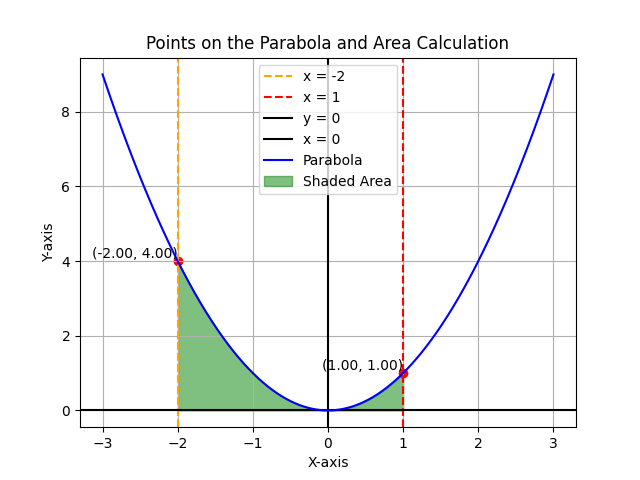
\includegraphics[width=0.8\textwidth]{figs/fig.png} % Ensure the image exists
\end{figure}
\end{frame}

\begin{frame}[fragile, allowframebreaks]{C Code: Area and Points on the Curve}
\lstset{
        language = C,
        basicstyle=\ttfamily\tiny,
        keywordstyle=\color{blue},
        stringstyle=\color{green},
        commentstyle=\color{gray},
        tabsize=4
    }
    \lstinputlisting{./codes/area_calculator.c}
\end{frame}

\begin{frame}[fragile, allowframebreaks]{Python: To plot the points}
\lstset{
        language = Python,
        basicstyle=\ttfamily\tiny,
        keywordstyle=\color{blue},
        stringstyle=\color{green},
        commentstyle=\color{gray},
        tabsize=4
    }
    \lstinputlisting{./codes/plot.py}
\end{frame}

\end{document}

